\documentclass[10pt,handout]{beamer}
\usetheme[
%%% options passed to the outer theme
%    hidetitle,           % hide the (short) title in the sidebar
%    hideauthor,          % hide the (short) author in the sidebar
%    hideinstitute,       % hide the (short) institute in the bottom of the sidebar
%    shownavsym,          % show the navigation symbols
%    width=2cm,           % width of the sidebar (default is 2 cm)
%    hideothersubsections,% hide all subsections but the subsections in the current section
%    hideallsubsections,  % hide all subsections
%    right                % right of left position of sidebar (default is right)
  ]{Aalborg}

\definecolor{aaublue}{RGB}{33,26,82}
\definecolor{aaugrey}{RGB}{84,97,110}

% If you want to change the colors of the various elements in the theme, edit and uncomment the following lines
% Change the bar and sidebar colors:
\setbeamercolor{Aalborg}{fg=aaublue!10,bg=aaugrey!60}
%\setbeamercolor{sidebar}{bg=blue!74}
% Change the color of the structural elements:
\setbeamercolor{structure}{fg=aaublue}
 \setbeamercolor{subtitle}{fg=aaugrey}
% Change the frame title text color:
\setbeamercolor{frametitle}{fg=aaublue}
% Change the normal text color background:
%\setbeamercolor{normal text}{bg=aaugrey!10}
% ... and you can of course change a lot more - see the beamer user manual.
\usebackgroundtemplate{
\includegraphics[width=\paperwidth]{img/background}}

\usepackage[utf8]{inputenc}
\usepackage[english]{babel}
\usepackage[T1]{fontenc}
\usepackage{soul} % use this (many fancier options)
\DeclareUnicodeCharacter{00A0}{~} % Fixes the "! Package inputenc Error: Unicode char \u8:  not set up for use with LaTeX."
% ... or whatever. Note that the encoding and the font should match. If T1
% does not look nice, try deleting the line with the fontenc.
\usepackage{lmodern} %optional

% colored hyperlinks
\newcommand{\chref}[2]{%
  \href{#1}{{\usebeamercolor[bg]{Aalborg}#2}}
}

\title[AAUSHIP Formation Control]% optional, use only with long paper titles
{Halfway Statusseminar for the\\ AAUSHIP Formation Control Project}

%\subtitle[v.\ 0.1.1] %optional
%{v.\ 0.1.1}

\author[14gr1034]{% optionally input the group number, use only with lots of authors
  Nick Østergaard \and Jeppe Dam\\
  {{\tt \{nickoe,jeppedam\}@es.aau.dk}}
}
% - Give the names in the same order as they appear in the paper.
% - Use the \inst{?} command only if the authors have different
%   affiliation. See the beamer manual for an example

%specify some optional logos
\pgfdeclareimage[height=1.2cm]{mainlogo}{aau_logo.pdf} % placed in the upper left/right corner
\logo{\pgfuseimage{mainlogo}}

\pgfdeclareimage[height=0.75cm]{logo2}{tu-logo} % placed in the lower left/right corner if the \pgfuseimage{logo2} command is uncommented in the \institute command below

\institute[
%  {\pgfuseimage{logo2}}\\ %insert a company or department logo
  Dept.\ of Electronic Systems,\\
  Aalborg University,\\
  Denmark
] % optional - is placed in the bottom of the sidebar on every slide
{%
  Department of Electronic Systems,\\
  Aalborg University,\\
  Denmark
  
  %there must be an empty line above this line - otherwise some unwanted space is added between the university and the country (I do not know why;( )
}
\date{\today}

\begin{document}
% the titlepage
\begin{frame}[plain] % the plain option removes the sidebar and header from the title page
  \titlepage
\end{frame}
%%%%%%%%%%%%%%%%

% TOC
\begin{frame}{Agenda}{}
\tableofcontents
\end{frame}
%%%%%%%%%%%%%%%%
\section{Introduction}
\begin{frame}{Introduction}{Motivation}
  \begin{itemize}
  	\item<1-> Little to no research are currently devoted to maritime autonomous crafts.
    \item<2-> During the 2012 Fukushima accident in Japan, no measurements of the spread of radioactivity was available in the coastal zones, thus relying only on estimates. 
    \item<3-> The coastal area around Greenland has no up-to-date baymethric maps available, and with the growing interest in Greenland (both industrially and commercially) this poses a threat to the ships going in and out of the fjords.
  \end{itemize}
\end{frame}

%%%%%%%%%%%%%%%%
\section{Development}
\subsection{AAUSHIP.01}
\begin{frame}{Development}{AAUSHIP.01}
\begin{itemize}
	\item<1-> The ship is designed as a non-planing deplacement craft (eg. like freight ships).
	\item<2-> Developed using rapid prototyping techniques.
	\item<3-> Developed in Rhinoceros\texttrademark using a lofting techniques.
	\item<4-> Printed on a 3D printer.
	\item<5-> Examined and the process iterated.
	\item<6-> Vaccumformed by DD-plast in Randers and assembled in the machine shop at Aalborg University.
\end{itemize}
\end{frame}

%%%%%%%%%%%%%%%%
\begin{frame}{Development}{AAUSHIP.01 Hull}
\begin{figure}
	\begin{center}
		%\includegraphics[width=8.2cm]{img/rendermontage}
		\label{fig:render}
	\end{center}
\end{figure}
\end{frame}

%%%%%%%%%%%%%%%%
\begin{frame}{Development}{AAUSHIP.01 Hull}
\begin{figure}
	\begin{center}
		%\includegraphics[width=8.2cm]{img/VerticalJumpingTele}
		\label{fig:jumping}
	\end{center}
\end{figure}
\end{frame}

%%%%%%%%%%%%%%%%
\subsection{Development}
\begin{frame}{Development}{Hardware}
\begin{itemize}
	\item Fitted with 2 x 1200W engines (totally producing around 3 HP at full thrust).
	\item Fitted with 6 x 3200mAh batteries (results in a mission time of around 5 hours).
	\item 2 counter rotating 60mm propellers.
	\item Inertial Measurement Unit.
	\item Global Positioning System.
	\item A (currently) 20mW 19.2 kbps radio link @ 470 MHz
	\item Arduino Mega with a custom made shield board mounted.
    \item Retrofitted with a hydrofoil to reduce the wake and pitch of the ship.
\end{itemize}
\end{frame}


%###########################
\begin{frame}{Testing the control algorithms}{Results}
	\begin{itemize}
	\item Plot of the ship states during the voyage
	\end{itemize}
	\begin{figure}
		\begin{center}
			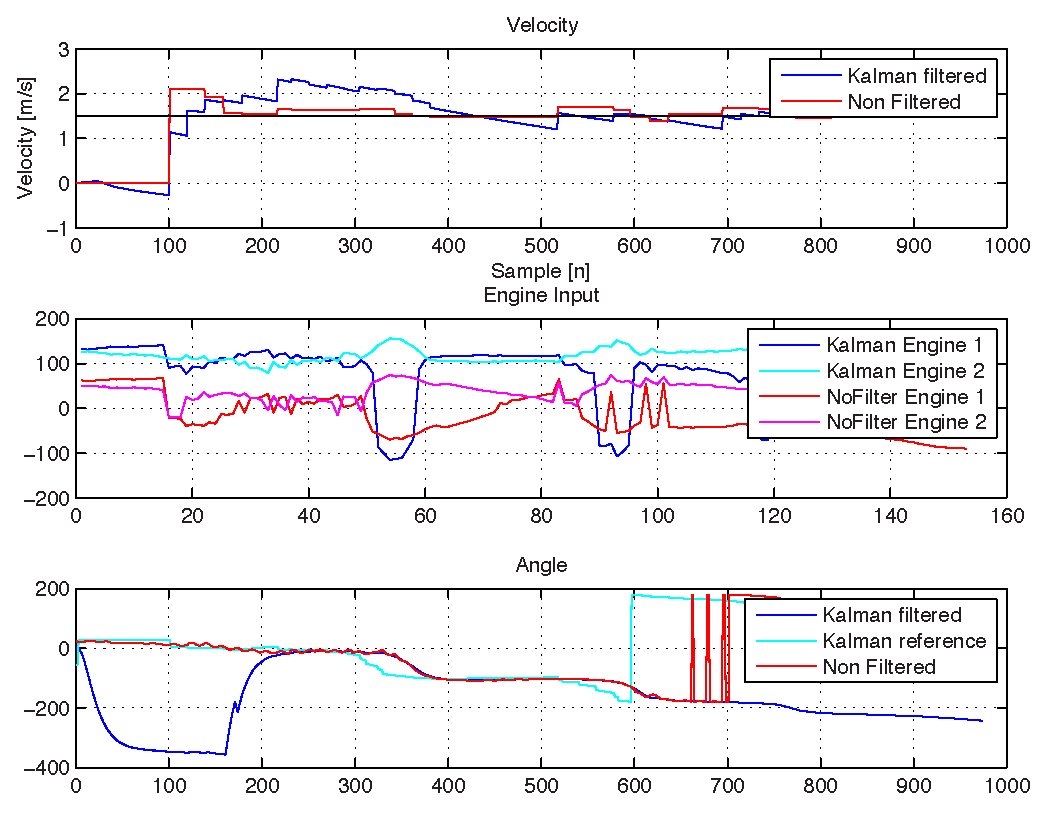
\includegraphics[width=8.2cm]{img/states}
			\label{fig:controltest3}
		\end{center}
	\end{figure}
\end{frame}

{
\setbeamertemplate{background canvas}{\centering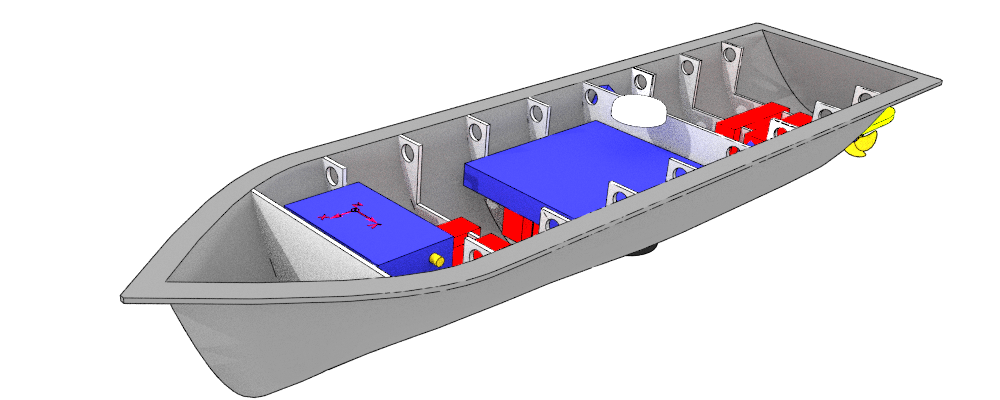
\includegraphics[height=\paperheight,keepaspectratio]{{img/aauship}}}
\begin{frame}[plain]{}\end{frame}}

\end{document}
